\section{RF/Microwave Components and Devices}
{\color{sub}\footnotesize 8 hrs \gap$\cdot$\gap asked in \mk{all 24 papers}
\gap$\cdot$\gap 11 syllabus sub-topics \gap$\cdot$\gap \mk{317 marks, 16.7\% of the archive,
52 questions}
$\rightarrow$ one derivation (the waveguide) worth up to 10 marks, one device (the magic tee)
asked 9 times, and a ring of 4 to 6 mark short notes.}

\vspace{3pt}\noindent
\colorbox{gdL}{\makebox[\dimexpr\textwidth-2\fboxsep][l]{%
  \textcolor{gd}{\bfseries\footnotesize READ THIS FIRST}}}
\par\nobreak\vspace{3pt}

Chapter 4 has the biggest question count in the paper, but three scripts answer most of it:
\begin{enumerate}[label=\arabic*., leftmargin=1.4em, itemsep=1pt]
  \item \textbf{Field equations of a rectangular waveguide, TE or TM} (14 papers, up to
    \mk{10 marks}) $\rightarrow$ $\S$4.1. \mk{One six-step script covers both modes}: only
    the boundary condition in step 4 changes. Learn TM first; TE is the same page with
    $\sin$ and $\cos$ swapped.
  \item \textbf{Mode questions} (9 papers, 1 to 5 marks each): dominant, degenerate, ``prove
    TM$_{01}$ cannot exist'', ``show TM$_{11}$ is the lowest TM mode'' $\rightarrow$ $\S$4.2.
    Every one is \mk{the cut-off formula plus one sentence}.
  \item \textbf{Magic tee} (9 papers) $\rightarrow$ $\S$4.5 for construction and the
    derivation, $\S$3.6 for the matrix. The combinations (two tees joined, arms terminated)
    are worked in the numerical companion.
\end{enumerate}
Two more things worth knowing before the paper starts:
\begin{itemize}
  \item \textbf{Circular waveguide} (4 papers, 7 to 10 marks) is the rectangular script
    again in cylindrical coordinates, with Bessel functions in place of sines. The only new
    fact to memorise is the \textbf{root table} of $\S$4.3.
  \item \textbf{Short notes} rotate among circulator (3 papers), directional coupler
    (3), cavity resonator (2), Gunn diode, MASER, probe/loop coupling and microstrip (1 each).
    Each gets a ready answer below.
\end{itemize}

\hr

%=======================================================================
\T{4.1 Rectangular Waveguide: TE and TM Field Equations}

\Q{Derive the field equations and characteristic parameters of a rectangular waveguide operating in TE / TM mode}{\m{4}\m{5}\m{7+3}\m{8}\m{8+2}\m{10}}
{\color{sub}\footnotesize \tS{14} \yr{\textbf{69 Bh}, \textbf{70 Bh}, 70 Ma, \textbf{71 Bh}, 72 Ma, 74 Ma, \textbf{74 Bh}, \textbf{76 Bh}, \textbf{77 Ch}, \textbf{79 Ch}, \textbf{80 Ch}, \textbf{\texttt{80 Bh}}, \texttt{81 Ba}, \textbf{\texttt{81 Bh}}} \gap$\cdot$\gap \mk{the most repeated ask in the chapter: TE 6 papers, TM 7, modes in general 1}}

\sbsr{0.56}{%
\lead{Set-up}
\begin{itemize}
  \item Hollow metal pipe, inner broad wall $a$ along $x$, narrow wall $b$ along $y$,
    propagation along $+z$, $a > b$.
  \item Lossless dielectric $(\mu, \epsilon)$ inside, perfectly conducting walls.
  \item Every field component carries $e^{-\gamma z}$, $\gamma = \alpha + j\beta$.
  \item Notation used throughout (Gangaju):
  \begin{itemize}
    \item $k = \omega\sqrt{\mu\epsilon}$, the free-space wave number of the filling.
    \item $h^2 = \gamma^2 + k^2 = k_x^2 + k_y^2$, the cut-off wave number squared
      (Pozar writes $k_c^2$).
  \end{itemize}
  \item \textbf{No TEM mode.} With $E_z = H_z = 0$ every transverse component below is
    zero. Physically, a closed $H$ loop in the cross-section needs an axial current, and a
    single hollow conductor has no centre conductor to carry it.
\end{itemize}}{%
\figT{c4_rect_geom.png}
{\color{sub}\scriptsize Co-ordinates of the rectangular guide. Source: Gangaju, Ch-4 deck, slide 12.}}

\lead{Step 1: transverse fields from the longitudinal ones (Maxwell's curl equations)}
\begin{itemize}
  \item Write $\nabla\times E = -j\omega\mu H$ and $\nabla\times H = j\omega\epsilon E$ in
    components with $\partial/\partial z \rightarrow -\gamma$, and solve the four transverse
    equations for $E_x, E_y, H_x, H_y$:
\end{itemize}
\[
\begin{aligned}
E_x &= -\frac{\gamma}{h^2}\frac{\partial E_z}{\partial x} - \frac{j\omega\mu}{h^2}\frac{\partial H_z}{\partial y}, &
E_y &= -\frac{\gamma}{h^2}\frac{\partial E_z}{\partial y} + \frac{j\omega\mu}{h^2}\frac{\partial H_z}{\partial x}, \\[3pt]
H_x &= -\frac{\gamma}{h^2}\frac{\partial H_z}{\partial x} + \frac{j\omega\epsilon}{h^2}\frac{\partial E_z}{\partial y}, &
H_y &= -\frac{\gamma}{h^2}\frac{\partial H_z}{\partial y} - \frac{j\omega\epsilon}{h^2}\frac{\partial E_z}{\partial x}.
\end{aligned}
\]
\begin{itemize}
  \item \mk{This block is the whole trick}: find $E_z$ (TM) or $H_z$ (TE) and the other four
    components follow by differentiation.
\end{itemize}

\lead{Step 2: the wave equation for the longitudinal component}
\begin{itemize}
  \item Helmholtz: $\nabla^2 E_z + k^2 E_z = 0$, i.e.
    $\dfrac{\partial^2 E_z}{\partial x^2} + \dfrac{\partial^2 E_z}{\partial y^2}
    + \dfrac{\partial^2 E_z}{\partial z^2} + \omega^2\mu\epsilon E_z = 0$.
  \item The same equation holds for $H_z$.
\end{itemize}

\lead{Step 3: separation of variables}
\begin{itemize}
  \item Put $E_z = X(x)\,Y(y)\,Z(z)$ and divide by $XYZ$:
    $\dfrac{X''}{X} + \dfrac{Y''}{Y} + \dfrac{Z''}{Z} = -k^2$.
  \item Each ratio must be a constant:
  \begin{itemize}
    \item $X''/X = -k_x^2 \Rightarrow X = C_1\cos k_x x + C_2\sin k_x x$.
    \item $Y''/Y = -k_y^2 \Rightarrow Y = C_3\cos k_y y + C_4\sin k_y y$.
    \item $Z''/Z = \gamma^2 \Rightarrow Z = C_5 e^{\gamma z} + C_6 e^{-\gamma z}$;
      a wave along $+z$ only $\Rightarrow C_5 = 0$.
  \end{itemize}
  \item Adding the constants back: $-k_x^2 - k_y^2 + \gamma^2 = -k^2$, so
    $\boxed{h^2 = k_x^2 + k_y^2 = \gamma^2 + k^2}$.
  \item General solution:
    $E_z = (A_1\cos k_x x + A_2\sin k_x x)(A_3\cos k_y y + A_4\sin k_y y)\,e^{-\gamma z}$.
  \item $H_z$ has the same form with its own constants $B_1, B_2, B_3, B_4$; the
    working below reuses the letters $A$ for brevity.
\end{itemize}

\par\penalty0\Needspace{16\baselineskip}
\sbs{%
\lead{Step 4 (TM): $H_z = 0$, apply $E_z = 0$ on the walls}
\begin{itemize}
  \item $E_z$ is tangential to every wall, so it must vanish there.
  \item $x = 0$: $E_z = 0 \Rightarrow A_1 = 0$.
  \item $y = 0$: $E_z = 0 \Rightarrow A_3 = 0$.
  \item $x = a$: $\sin k_x a = 0 \Rightarrow k_x = m\pi/a$.
  \item $y = b$: $\sin k_y b = 0 \Rightarrow k_y = n\pi/b$.
\end{itemize}
\[ E_z = E_0 \sin\frac{m\pi x}{a}\,\sin\frac{n\pi y}{b}\,e^{-\gamma z} \]}{%
\lead{Step 4 (TE): $E_z = 0$, apply $E_x, E_y = 0$ on the walls}
\begin{itemize}
  \item With $E_z = 0$: $E_x \propto \partial H_z/\partial y$, $E_y \propto \partial H_z/\partial x$.
  \item $x = 0$: $E_y = 0 \Rightarrow \partial H_z/\partial x = 0 \Rightarrow A_2 = 0$.
  \item $y = 0$: $E_x = 0 \Rightarrow \partial H_z/\partial y = 0 \Rightarrow A_4 = 0$.
  \item $x = a$: $\sin k_x a = 0 \Rightarrow k_x = m\pi/a$.
  \item $y = b$: $\sin k_y b = 0 \Rightarrow k_y = n\pi/b$.
\end{itemize}
\[ H_z = H_0 \cos\frac{m\pi x}{a}\,\cos\frac{n\pi y}{b}\,e^{-\gamma z} \]
{\color{sub}\footnotesize Deck slide 18 prints $k_y = n\pi/a$ in the last line; it is $n\pi/b$.}}

\par\penalty0\Needspace{18\baselineskip}
\lead{Step 5: substitute into Step 1 (write $e^{-\gamma z}$ on every line in the exam)}
\sbs{%
\textbf{TM$_{mn}$} \quad ($H_z = 0$)
\[
\begin{aligned}
E_x &= -\frac{\gamma}{h^2}\frac{m\pi}{a}E_0\cos\frac{m\pi x}{a}\sin\frac{n\pi y}{b} \\
E_y &= -\frac{\gamma}{h^2}\frac{n\pi}{b}E_0\sin\frac{m\pi x}{a}\cos\frac{n\pi y}{b} \\
H_x &= \phantom{-}\frac{j\omega\epsilon}{h^2}\frac{n\pi}{b}E_0\sin\frac{m\pi x}{a}\cos\frac{n\pi y}{b} \\
H_y &= -\frac{j\omega\epsilon}{h^2}\frac{m\pi}{a}E_0\cos\frac{m\pi x}{a}\sin\frac{n\pi y}{b}
\end{aligned}
\]}{%
\textbf{TE$_{mn}$} \quad ($E_z = 0$)
\[
\begin{aligned}
E_x &= \phantom{-}\frac{j\omega\mu}{h^2}\frac{n\pi}{b}H_0\cos\frac{m\pi x}{a}\sin\frac{n\pi y}{b} \\
E_y &= -\frac{j\omega\mu}{h^2}\frac{m\pi}{a}H_0\sin\frac{m\pi x}{a}\cos\frac{n\pi y}{b} \\
H_x &= \phantom{-}\frac{\gamma}{h^2}\frac{m\pi}{a}H_0\sin\frac{m\pi x}{a}\cos\frac{n\pi y}{b} \\
H_y &= \phantom{-}\frac{\gamma}{h^2}\frac{n\pi}{b}H_0\cos\frac{m\pi x}{a}\sin\frac{n\pi y}{b}
\end{aligned}
\]}
{\color{sub}\footnotesize All eight components are checked in \code{src/wg.py} against both curl
equations and against tangential $E = 0$ on all four walls; a single flipped sign fails the
check.}

\par\penalty0\Needspace{20\baselineskip}
\lead{Step 6: the characteristic equations (the ``+2'' or ``+3'' of every version)}
\begin{tabularx}{\linewidth}{@{}L{3.1cm}L{6.1cm}X@{}}
\toprule
\hrow \thead{Quantity} & \thead{Expression} & \thead{Note} \\
\midrule
Propagation constant & $\gamma = \sqrt{h^2 - k^2} = \sqrt{\left(\tfrac{m\pi}{a}\right)^2 + \left(\tfrac{n\pi}{b}\right)^2 - \omega^2\mu\epsilon}$ & real below cut-off, imaginary above \\
Cut-off frequency & $f_c = \dfrac{1}{2\sqrt{\mu\epsilon}}\sqrt{\left(\tfrac{m}{a}\right)^2 + \left(\tfrac{n}{b}\right)^2}$ & set $\gamma = 0$; air: $\tfrac{c}{2}\sqrt{\cdot}$ \\
Cut-off wavelength & $\lambda_c = \dfrac{2}{\sqrt{(m/a)^2 + (n/b)^2}}$ & TE$_{10}$: $\lambda_c = 2a$ \\
Phase constant & $\beta = \omega\sqrt{\mu\epsilon}\sqrt{1 - (f_c/f)^2}$ & above cut-off \\
Guide wavelength & $\lambda_g = \dfrac{\lambda}{\sqrt{1 - (f_c/f)^2}}$ & $\dfrac{1}{\lambda^2} = \dfrac{1}{\lambda_g^2} + \dfrac{1}{\lambda_c^2}$ \\
Phase velocity & $v_p = \dfrac{\omega}{\beta} = \dfrac{v}{\sqrt{1 - (f_c/f)^2}}$ & $> v$, carries no energy \\
Group velocity & $v_g = \dfrac{d\omega}{d\beta} = v\sqrt{1 - (f_c/f)^2}$ & $< v$; $v_p v_g = v^2$ \\
Wave impedance, TE & $Z_{TE} = \dfrac{E_x}{H_y} = -\dfrac{E_y}{H_x} = \dfrac{\omega\mu}{\beta} = \dfrac{\eta}{\sqrt{1 - (f_c/f)^2}}$ & $> \eta$ \\
Wave impedance, TM & $Z_{TM} = \dfrac{E_x}{H_y} = -\dfrac{E_y}{H_x} = \dfrac{\beta}{\omega\epsilon} = \eta\sqrt{1 - (f_c/f)^2}$ & $< \eta$ \\
\bottomrule
\end{tabularx}
\vspace{2pt}
\begin{itemize}
  \item Three regimes from $\gamma^2 = h^2 - \omega^2\mu\epsilon$:
  \begin{itemize}
    \item $f < f_c$: $\gamma = \alpha$, real $\rightarrow$ \textbf{evanescent}, the field
      decays and carries no power. A waveguide is a \textbf{high-pass filter}.
    \item $f = f_c$: $\gamma = 0$, cut-off.
    \item $f > f_c$: $\gamma = j\beta$ $\rightarrow$ \textbf{propagates}.
  \end{itemize}
  \item $v = 1/\sqrt{\mu\epsilon}$, $\eta = \sqrt{\mu/\epsilon}$; for air $v = c$ and
    $\eta_0 = 120\pi \approx 377\,\Omega$.
\end{itemize}

\par\penalty0\Needspace{12\baselineskip}
\creamq{Answer skeleton for the 4 to 5 mark short-note version}{\m{4}\m{5}}
\begin{itemize}
  \item Figure of the guide with $a$, $b$, $z$ (1 line).
  \item Step 1 block, then the one boundary-condition result ($E_z = E_0\sin\sin$ for TM,
    $H_z = H_0\cos\cos$ for TE).
  \item The four transverse components from Step 5, without re-deriving them.
  \item $f_c$ and one of $Z_{TE}$ / $Z_{TM}$. For the 10-mark version add Steps 2 to 4 in
    full and the whole Step 6 table.
\end{itemize}

\penalty0\vspace{2pt}

%=======================================================================
\T{4.2 Modes: Dominant, Degenerate, and the Short Proofs}

\Q{Dominant and degenerate modes; show which modes cannot exist; compare modes by cut-off}{\m{1+1+2}\m{2}\m{2+2}\m{3}\m{5}}
{\color{sub}\footnotesize \tS{9} \yr{\textbf{70 Bh}, 70 Ma, \textbf{71 Bh}, 72 Ma, \textbf{72 Ash}, \textbf{\texttt{80 Bh}}, \textbf{\texttt{81 Bh}}, \texttt{82 Ba}, \textbf{\texttt{82 Bh}}} \gap$\cdot$\gap every one is the $f_c$ formula plus one sentence}

\sbs{%
\lead{Definitions}
\begin{itemize}
  \item \textbf{Mode}: one allowed field pattern, labelled by the integers $m, n$ =
    number of half-cycle variations across $a$ and across $b$.
  \item \textbf{Dominant mode}: the mode with the \textbf{lowest cut-off frequency}.
  \begin{itemize}
    \item Rectangular guide ($a > b$): \mk{TE$_{10}$}, $f_c = c/2a$, $\lambda_c = 2a$.
    \item Circular guide: \mk{TE$_{11}$}, $f_c = 1.841\,c/2\pi r$ ($\S$4.3).
    \item Between $f_{c,10}$ and the next cut-off only the dominant mode propagates
      $\rightarrow$ \textbf{single-mode} operation, the reason guides are sized this way.
  \end{itemize}
\end{itemize}}{%
\figT{c4_te_patterns.png}
{\color{sub}\scriptsize E and H field of TE$_{10}$, TE$_{20}$, TE$_{01}$: one, two and one
half-cycles across the walls. Source: Gangaju, slide 20.}}

\sbs{%
\begin{itemize}
  \item \textbf{Degenerate modes}: \textbf{different} field patterns with the \textbf{same}
    cut-off frequency.
  \begin{itemize}
    \item TE$_{mn}$ and TM$_{mn}$ for every $m, n \ge 1$: same $f_c$ formula.
    \item Square guide ($a = b$): TE$_{10}$ and TE$_{01}$ as well.
    \item Circular guide: TE$_{01}$ and TM$_{11}$ (both root 3.832).
    \item Unwanted, because power can couple between them at any discontinuity.
  \end{itemize}
\end{itemize}}{%
\figT{c4_cutoff_line.png}
{\color{sub}\scriptsize Cut-off ladder, Gangaju slide 22 (from Sadiku). The slide's caption
says $a = 2.5$ cm, $b = 1$ cm; the arrows (TE$_{10}$ at 3 GHz, TE$_{20}$ at 6,
TE$_{50}$ and TE$_{02}$ at 15) are those of a \textbf{5 cm $\times$ 2 cm} guide.
TM arrows below the line sit on their TE twins: degeneracy. \added{}}}

\par\penalty0\Needspace{10\baselineskip}
\creamq{Prove that TM$_{01}$ and TM$_{10}$ modes do not exist}{\m{3}}
{\color{sub}\footnotesize \yr{70 Ma}}
\begin{itemize}
  \item TM: $H_z = 0$ and $E_z = E_0\sin(m\pi x/a)\sin(n\pi y/b)e^{-\gamma z}$.
  \item $m = 0$ or $n = 0$ $\Rightarrow$ $\sin 0 = 0$ $\Rightarrow$ $E_z = 0$ everywhere.
  \item Every transverse component is a derivative of $E_z$ (Step 1 with $H_z = 0$)
    $\Rightarrow$ $E_x = E_y = H_x = H_y = 0$.
  \item All six components vanish $\Rightarrow$ \mk{no field, no mode}. TM$_{mn}$ needs
    $m \ge 1$ \textbf{and} $n \ge 1$.
\end{itemize}

\par\penalty0\Needspace{9\baselineskip}
\creamq{Prove that the lowest cut-off TM mode is TM$_{11}$}{\m{3}}
{\color{sub}\footnotesize \yr{\textbf{\texttt{82 Bh}}}}
\begin{itemize}
  \item From above, TM needs $m, n \ge 1$.
  \item $f_c = \frac{c}{2}\sqrt{(m/a)^2 + (n/b)^2}$ grows with both $m$ and $n$.
  \item Smallest admissible pair is $m = n = 1$:
    $\boxed{f_{c,TM_{11}} = \frac{c}{2}\sqrt{\frac{1}{a^2} + \frac{1}{b^2}}}$, for any $a, b$.
\end{itemize}

\par\penalty0\Needspace{15\baselineskip}
\creamq{Show that the dominant TE mode is TE$_{10}$; compare TE$_{10}$ with TE$_{20}$}{\m{2}\m{3}}
{\color{sub}\footnotesize \yr{\textbf{71 Bh}, \textbf{\texttt{81 Bh}}}}
\sbs{%
\begin{itemize}
  \item TE: $H_z = H_0\cos\cos$ survives with one index zero ($\cos 0 = 1$); only
    TE$_{00}$ is excluded (constant $H_z$, all transverse components zero).
  \item Two candidates for the lowest $f_c$:
    $f_{c,10} = \dfrac{c}{2a}$, \quad $f_{c,01} = \dfrac{c}{2b}$.
  \item $a > b \Rightarrow f_{c,10} < f_{c,01}$ $\Rightarrow$ \mk{TE$_{10}$ is dominant}.
    It also beats TM$_{11}$, since $\frac{1}{a^2} < \frac{1}{a^2} + \frac{1}{b^2}$.
  \item \textbf{81 Bh prints ``when $b > a$''.} With $b > a$ it is TE$_{01}$ that is
    dominant; TE$_{10}$ needs $a > b$. The paper has the inequality reversed. Prove the
    $a > b$ case and state this. \added{}
\end{itemize}}{%
\begin{tabularx}{\linewidth}{@{}L{1.9cm}XX@{}}
\toprule
\hrow & \thead{TE$_{10}$} & \thead{TE$_{20}$} \\
\midrule
$f_c$ & $c/2a$ & $c/a = 2f_{c,10}$ \\
$\lambda_c$ & $2a$ & $a$ \\
Variation across $a$ & one half-cycle & two half-cycles \\
Field components & $E_y, H_x, H_z$ only & same three \\
Status & \mk{dominant} & higher-order \\
\bottomrule
\end{tabularx}
\vspace{2pt}
\begin{itemize}
  \item Single-mode band: $c/2a < f < c/a$ provided $a \ge 2b$ (otherwise TE$_{01}$
    arrives first at $c/2b$).
\end{itemize}}

\par\penalty0\Needspace{11\baselineskip}
\creamq{Dominant vs degenerate modes; for $a = 3b$ find the dominant mode among TM$_{01}$, TM$_{10}$, TM$_{11}$, TM$_{21}$, TM$_{12}$, TM$_{02}$, TM$_{20}$}{\m{2+2}\m{3}}
{\color{sub}\footnotesize \yr{72 Ma, \texttt{82 Ba}} \gap$\cdot$\gap full working in the companion, Problem 4}
\begin{itemize}
  \item With $a = 3b$: $f_c = \dfrac{c}{2a}\sqrt{m^2 + 9n^2}$.
  \item TM$_{01}$, TM$_{10}$, TM$_{02}$, TM$_{20}$ \textbf{do not exist} (an index is zero).
  \item TM$_{11}$: $\sqrt{10} = 3.162$; TM$_{21}$: $\sqrt{13} = 3.606$;
    TM$_{12}$: $\sqrt{37} = 6.083$ (in units of $c/2a$).
  \item \mk{Dominant among those listed: TM$_{11}$.} (Overall, TE$_{10}$ at 1 unit.)
\end{itemize}

\par\penalty0\Needspace{9\baselineskip}
\creamq{Cut-off checks: does the guide pass the signal?}{\m{1+1+2}\m{3}\m{5}}
{\color{sub}\footnotesize \yr{\textbf{70 Bh}, \textbf{72 Ash}, \textbf{\texttt{80 Bh}}} \gap$\cdot$\gap worked in the companion, Problem 3}
\begin{itemize}
  \item Rule: compute $f_c$ of the \textbf{dominant} mode; the signal propagates only if
    $f > f_c$.
  \item \textbf{70 Bh}: wall separation 5 cm, TE$_{10}$: $f_c = 3$ GHz $> 1$ GHz
    $\Rightarrow$ \mk{1 GHz cannot propagate}; it decays at $59.2$ Np/m.
  \item \textbf{\texttt{80 Bh}}: width 2.254 cm: $f_c = 6.65$ GHz $> 6$ GHz $\Rightarrow$
    \mk{6 GHz is not supported}.
\end{itemize}

\penalty0\vspace{2pt}

%=======================================================================
\T{4.3 Circular Waveguide}

\Q{Field equations of a circular waveguide in TE / TM mode; TE vs TM; dominant mode}{\m{7}\m{8+2}\m{10}}
{\color{sub}\footnotesize \tF{4} \yr{71 Ma, \textbf{75 Bh}, \textbf{\texttt{79 Bh}}, \texttt{82 Ba}} \gap$\cdot$\gap the rectangular script in cylindrical co-ordinates}

\lead{Set-up}
\begin{itemize}
  \item Hollow circular pipe of inner radius $a$, co-ordinates $(\rho, \phi, z)$,
    fields $\propto e^{-j\beta z}$; $k_c^2 = k^2 - \beta^2$, with $k = \omega\sqrt{\mu\epsilon}$.
  \item \textbf{Step 1}, the cylindrical version of the transverse equations
    (Waveguide.pdf p8, Pozar $\S$3.4):
\end{itemize}
\[
\begin{aligned}
E_\rho &= -\frac{j}{k_c^2}\left(\beta\frac{\partial E_z}{\partial\rho} + \frac{\omega\mu}{\rho}\frac{\partial H_z}{\partial\phi}\right), &
E_\phi &= -\frac{j}{k_c^2}\left(\frac{\beta}{\rho}\frac{\partial E_z}{\partial\phi} - \omega\mu\frac{\partial H_z}{\partial\rho}\right), \\
H_\rho &= \phantom{-}\frac{j}{k_c^2}\left(\frac{\omega\epsilon}{\rho}\frac{\partial E_z}{\partial\phi} - \beta\frac{\partial H_z}{\partial\rho}\right), &
H_\phi &= -\frac{j}{k_c^2}\left(\omega\epsilon\frac{\partial E_z}{\partial\rho} + \frac{\beta}{\rho}\frac{\partial H_z}{\partial\phi}\right).
\end{aligned}
\]

\sbsr{0.40}{%
\figT{c4_circ_cavity.png}
{\color{sub}\scriptsize Cylindrical co-ordinates. The figure is a circular cavity (a guide
closed at both ends, $\S$4.8); the guide itself is the same cylinder, open along $z$.
Source: Gangaju, slide 93.}}{%
\lead{Step 2 and 3: separate the Helmholtz equation}
\begin{itemize}
  \item $\dfrac{\partial^2 h_z}{\partial\rho^2} + \dfrac{1}{\rho}\dfrac{\partial h_z}{\partial\rho}
    + \dfrac{1}{\rho^2}\dfrac{\partial^2 h_z}{\partial\phi^2} + k_c^2 h_z = 0$.
  \item $h_z = R(\rho)P(\phi)$:
  \begin{itemize}
    \item $P'' + n^2 P = 0 \Rightarrow P = A\sin n\phi + B\cos n\phi$; $n$ an
      \textbf{integer} because the field repeats every $2\pi$.
    \item $\rho^2R'' + \rho R' + (k_c^2\rho^2 - n^2)R = 0$: \textbf{Bessel's equation}
      $\Rightarrow R = C J_n(k_c\rho) + D Y_n(k_c\rho)$.
    \item $Y_n \rightarrow \infty$ at $\rho = 0$ $\Rightarrow$ $D = 0$.
  \end{itemize}
\end{itemize}}

\par\penalty0\Needspace{20\baselineskip}
\sbs{%
\lead{TE$_{nm}$: $E_z = 0$}
\begin{itemize}
  \item $H_z = (A\sin n\phi + B\cos n\phi)\,J_n(k_c\rho)\,e^{-j\beta z}$.
  \item \textbf{Boundary}: $E_\phi(\rho = a) = 0$. Since $E_\phi \propto \partial H_z/\partial\rho$:
    $J_n'(k_c a) = 0 \Rightarrow \boxed{k_c = p'_{nm}/a}$, $p'_{nm}$ = $m$-th root of $J_n'$.
\end{itemize}
\[
\begin{aligned}
E_\rho &= \frac{-j\omega\mu n}{k_c^2\rho}(A\cos n\phi - B\sin n\phi)J_n(k_c\rho) \\
E_\phi &= \frac{j\omega\mu}{k_c}(A\sin n\phi + B\cos n\phi)J_n'(k_c\rho) \\
H_\rho &= \frac{-j\beta}{k_c}(A\sin n\phi + B\cos n\phi)J_n'(k_c\rho) \\
H_\phi &= \frac{-j\beta n}{k_c^2\rho}(A\cos n\phi - B\sin n\phi)J_n(k_c\rho)
\end{aligned}
\]
\begin{itemize}
  \item $f_{c} = \dfrac{p'_{nm}}{2\pi a\sqrt{\mu\epsilon}}$, \quad
    $Z_{TE} = \dfrac{E_\rho}{H_\phi} = \dfrac{\omega\mu}{\beta} = \dfrac{\eta k}{\beta}$.
\end{itemize}}{%
\lead{TM$_{nm}$: $H_z = 0$}
\begin{itemize}
  \item $E_z = (A\sin n\phi + B\cos n\phi)\,J_n(k_c\rho)\,e^{-j\beta z}$.
  \item \textbf{Boundary}: $E_z(\rho = a) = 0$ directly:
    $J_n(k_c a) = 0 \Rightarrow \boxed{k_c = p_{nm}/a}$, $p_{nm}$ = $m$-th root of $J_n$.
\end{itemize}
\[
\begin{aligned}
E_\rho &= \frac{-j\beta}{k_c}(A\sin n\phi + B\cos n\phi)J_n'(k_c\rho) \\
E_\phi &= \frac{-j\beta n}{k_c^2\rho}(A\cos n\phi - B\sin n\phi)J_n(k_c\rho) \\
H_\rho &= \frac{j\omega\epsilon n}{k_c^2\rho}(A\cos n\phi - B\sin n\phi)J_n(k_c\rho) \\
H_\phi &= \frac{-j\omega\epsilon}{k_c}(A\sin n\phi + B\cos n\phi)J_n'(k_c\rho)
\end{aligned}
\]
\begin{itemize}
  \item $f_{c} = \dfrac{p_{nm}}{2\pi a\sqrt{\mu\epsilon}}$, \quad
    $Z_{TM} = \dfrac{E_\rho}{H_\phi} = \dfrac{\beta}{\omega\epsilon} = \dfrac{\eta\beta}{k}$.
  \item \mk{Sign}: Waveguide.pdf p11 prints $E_\phi$ with a $+$; it is $-$.
    \code{wg.py} fails the curl equation with the $+$. \added{}
\end{itemize}}

\par\penalty0\Needspace{14\baselineskip}
\sbs{%
\lead{Root table and mode order (all a circular answer needs)}
\begin{tabularx}{\linewidth}{@{}L{1.3cm}L{1.9cm}L{1.9cm}X@{}}
\toprule
\hrow \thead{Mode} & \thead{Root} & \thead{$\lambda_c$} & \thead{Order} \\
\midrule
TE$_{11}$ & $p'_{11} = 1.841$ & $3.41a$ & \mk{1st, dominant} \\
TM$_{01}$ & $p_{01} = 2.405$ & $2.61a$ & 2nd, lowest TM \\
TE$_{21}$ & $p'_{21} = 3.054$ & $2.06a$ & 3rd \\
TE$_{01}$ & $p'_{01} = 3.832$ & $1.64a$ & 4th (low-loss mode) \\
TM$_{11}$ & $p_{11} = 3.832$ & $1.64a$ & degenerate with TE$_{01}$ \\
\bottomrule
\end{tabularx}
\vspace{2pt}
{\color{sub}\footnotesize $\lambda_c = 2\pi a/p$. Roots from \code{scipy} in \code{wg.py}. Worked
example: $a = 2$ cm gives TE$_{11}$ at $4.40$ GHz and TM$_{01}$ at $5.74$ GHz (Waveguide.pdf p13).}}{%
\lead{TE vs TM in a circular guide (71 Ma)}
\begin{tabularx}{\linewidth}{@{}L{1.7cm}XX@{}}
\toprule
\hrow & \thead{TE$_{nm}$} & \thead{TM$_{nm}$} \\
\midrule
Longitudinal & $E_z = 0$, $H_z \ne 0$ & $H_z = 0$, $E_z \ne 0$ \\
Boundary & $J_n'(k_c a) = 0$ & $J_n(k_c a) = 0$ \\
Roots & $p'_{nm}$ & $p_{nm}$ \\
Dominant & TE$_{11}$, 1.841 & TM$_{01}$, 2.405 \\
Impedance & $\eta k/\beta > \eta$ & $\eta\beta/k < \eta$ \\
$m = 0$ ? & TE$_{n0}$ absent & TM$_{n0}$ absent \\
Special & TE$_{01}$: loss falls with $f$ & TM$_{01}$: symmetric, rotary joints \\
\bottomrule
\end{tabularx}
\vspace{2pt}
\begin{itemize}
  \item \textbf{75 Bh}: dominant TE mode = TE$_{11}$, dominant TM mode = TM$_{01}$, and
    TE$_{11}$ is dominant overall since $1.841 < 2.405$.
\end{itemize}}

\penalty0\vspace{2pt}

%=======================================================================
\T{4.4 Coupling Energy into a Waveguide: Probes, Loops and Slots}

\Q{Probe coupling vs loop coupling}{\m{5}}
{\color{sub}\footnotesize \tP{1} \yr{\textbf{69 Bh}} \gap$\cdot$\gap also the answer to ``how is a cavity or klystron excited''}

\sbsr{0.62}{%
\begin{tabularx}{\linewidth}{@{}L{1.55cm}XX@{}}
\toprule
\hrow & \thead{Probe} & \thead{Loop} \\
\midrule
Couples to & \textbf{E} field & \textbf{H} field \\
Acts as & quarter-wave monopole antenna & small magnetic dipole \\
Best position & centre of broad wall $a$, parallel to E lines, $\lambda_g/4$ from the shorted end (E maximum) & where H is strongest, e.g. at the shorted end; loop plane normal to H lines \\
Less coupling & shorten, move off centre, shield & rotate, or move to fewer H lines \\
Bandwidth & grows with probe diameter & grows with wire size \\
Power & door-knob probe: more area, more power & grows with loop diameter \\
Removal & same probe, reverse action & same loop, induced current \\
\bottomrule
\end{tabularx}}{%
\figT{c4_probe.png}
\vspace{2pt}

\figT{c4_loop.png}
{\color{sub}\scriptsize Probe (top) launches E lines; loop (bottom) links H lines. Source:
Gangaju, slides 3 and 6.}}
\begin{itemize}
  \item \textbf{Slot / aperture}: a hole in the wall where the field is strong; gives
    \textbf{loose} coupling, used between a guide and a cavity or a second guide
    (directional coupler, $\S$4.6).
  \item Choice depends on: voltage breakdown near an antinode, ease of adjustment,
    constancy of coupling under mechanical change, not disturbing an electron beam, matching.
\end{itemize}

\penalty0\vspace{2pt}

%=======================================================================
\T{4.5 Waveguide Tee Junctions and the Magic Tee}

\Q{Explain the magic tee with a neat diagram and derive its S-matrix; E-plane vs H-plane tee}{\m{3+3}\m{4}\m{5}\m{6}\m{8}}
{\color{sub}\footnotesize \tS{9} \yr{71 Ma, \textbf{71 Bh}, \textbf{72 Ash}, 72 Ma, \textbf{79 Ch}, \textbf{\texttt{79 Bh}}, \textbf{80 Ch}, \textbf{\texttt{80 Bh}}, \textbf{\texttt{82 Bh}}} \gap$\cdot$\gap the matrices are catalogued in $\S$3.6; this band adds construction, derivation and use}

\sbsr{0.42}{%
\figT{c3_magictee.png}
{\color{sub}\scriptsize Magic tee: collinear ports 1, 2; E-arm 3; H-arm 4.}}{%
\lead{Construction}
\begin{itemize}
  \item A \textbf{hybrid} of the two simple tees on one junction:
  \begin{itemize}
    \item \textbf{E-plane (series) tee}: side arm on the \textbf{broad} wall, its axis
      parallel to the main guide's E field. Port 3.
    \item \textbf{H-plane (shunt) tee}: side arm on the \textbf{narrow} wall, in the plane
      of H. Port 4.
  \end{itemize}
  \item Collinear arms 1 and 2 are symmetric about both side arms.
  \item A \textbf{post and iris} inside the junction match ports 3 and 4; without them the
    junction is simply a ``hybrid tee'' and is poorly matched.
  \item It is called \textbf{magic} because a matched 4-port with this symmetry turns out
    to be matched at \textbf{all} ports and isolates the two pairs, which nothing in its
    shape makes obvious.
\end{itemize}}

\par\penalty0\Needspace{20\baselineskip}
\lead{Derivation of the S-matrix, the 4-mark version asked in 80 Bh and 72 Ma}
\begin{enumerate}[label=\arabic*., leftmargin=1.4em, itemsep=1pt]
  \item 4 ports $\Rightarrow$ a $4\times4$ matrix $[S]$; write all sixteen $S_{ij}$ out,
    $i, j$ from 1 to 4.
  \item \textbf{H-arm symmetry}: input at 4 reaches 1 and 2 equally and \textbf{in phase}
    $\Rightarrow S_{14} = S_{24}$.
  \item \textbf{E-arm antisymmetry}: input at 3 reaches 1 and 2 equally and in
    \textbf{antiphase} $\Rightarrow S_{13} = -S_{23}$.
  \item \textbf{E and H arms are orthogonal}: an E-arm wave cannot excite the H-arm mode
    $\Rightarrow S_{34} = S_{43} = 0$.
  \item \textbf{Matched side arms} (post and iris) $\Rightarrow S_{33} = S_{44} = 0$.
  \item \textbf{Reciprocity} $\Rightarrow S_{ij} = S_{ji}$.
  \item \textbf{Unitary, column 3}: $|S_{13}|^2 + |S_{23}|^2 = 1$, with
    $|S_{13}| = |S_{23}| \Rightarrow S_{13} = 1/\sqrt{2}$. Same for column 4:
    $S_{14} = 1/\sqrt{2}$.
  \item \textbf{Unitary, column 1}: $|S_{11}|^2 + |S_{12}|^2 + \tfrac{1}{2} + \tfrac{1}{2} = 1
    \Rightarrow S_{11} = S_{12} = 0$; column 2 gives $S_{22} = 0$.
  \item Result:
    $\;[S] = \dfrac{1}{\sqrt{2}}\left[\begin{smallmatrix} 0&0&1&1\\ 0&0&-1&1\\ 1&-1&0&0\\ 1&1&0&0 \end{smallmatrix}\right]$,
    matched at all four ports, lossless, reciprocal.
\end{enumerate}

\par\penalty0\Needspace{16\baselineskip}
\sbs{%
\lead{Properties (read straight off the matrix)}
\begin{itemize}
  \item Into \textbf{H-arm} (4): equal halves at 1 and 2, \textbf{in phase}; nothing at 3.
  \item Into \textbf{E-arm} (3): equal halves at 1 and 2, \textbf{antiphase}; nothing at 4.
  \item Into \textbf{collinear} port 1: halves at 3 and 4; \textbf{nothing at 2}.
  \item Equal in-phase signals at 1 and 2: \textbf{sum} emerges at 4, nothing at 3.
  \item Equal antiphase signals at 1 and 2: \textbf{difference} emerges at 3, nothing at 4.
  \item All four ports matched: no reflection anywhere.
\end{itemize}
\lead{Applications}
\begin{itemize}
  \item Power combiner, e.g. two radar transmitters into one antenna ($\S$3.8).
  \item Duplexer: transmitter and receiver on the isolated E and H arms ($\S$3.6).
  \item Balanced mixer: signal on one side arm, local oscillator on the other.
  \item Impedance bridge / measurement: unknown and standard on 1 and 2, null detector on 3.
  \item Monopulse radar comparator: sum and difference channels.
\end{itemize}}{%
\lead{E-plane tee vs H-plane tee}
\begin{tabularx}{\linewidth}{@{}L{1.55cm}XX@{}}
\toprule
\hrow & \thead{E-plane (series)} & \thead{H-plane (shunt)} \\
\midrule
Side arm on & broad wall, $\parallel$ E & narrow wall, $\parallel$ H \\
Side-arm input & antiphase at 1, 2 & in phase at 1, 2 \\
Relation & $S_{13} = -S_{23}$ & $S_{13} = S_{23}$ \\
Equivalent & series junction & shunt junction \\
In-phase at 1, 2 & cancel in side arm & add in side arm \\
Matrix & $\S$3.6, $-1/\sqrt{2}$ in row 3 & $\S$3.6, $-1/2$ at $S_{12}$ \\
\bottomrule
\end{tabularx}
\vspace{2pt}
\begin{itemize}
  \item Both are 3-ports and \textbf{cannot} be lossless, reciprocal and matched at once
    ($\S$3.5): ports 1 and 2 stay mismatched with $|S_{11}| = 1/2$.
\end{itemize}
{\color{sub}\footnotesize \yr{\textbf{69 Bh} \m{5}, \texttt{80 Ba} \m{4}}}}

\sbsr{0.30}{%
\figT{c4_ratrace.png}}{%
\lead{Hybrid ring (rat race)}
\begin{itemize}
  \item Annular line, circumference $1.5\lambda_g$, four arms at $\lambda_g/4$,
    $\lambda_g/4$, $\lambda_g/4$ and $3\lambda_g/4$.
  \item Into port 1: the two ways round to port 3 differ by $\lambda_g/2$ (180$^\circ$)
    $\rightarrow$ cancel; to 2 and 4 they add. Same behaviour as a magic tee, in
    planar form, but only at the design frequency.
\end{itemize}}

\par\penalty0\Needspace{12\baselineskip}
\creamq{Tee combinations: arms terminated, two tees joined, a 3-port coupler}{\m{4}\m{4+4+2}\m{5}\m{8}\m{10}}
{\color{sub}\footnotesize \tF{5} \yr{70 Ma, \textbf{75 Bh}, \textbf{77 Ch}, \textbf{78 Ch}, \texttt{82 Ba}} \gap$\cdot$\gap each solved by connecting or terminating ports in \code{wg.py}; full working in the companion, Problems 6 to 8}
\begin{itemize}
  \item \textbf{Hybrid tee with a terminated arm} (\texttt{82 Ba}, 70 Ma): a matched load
    simply deletes that row and column.
  \begin{itemize}
    \item E-arm terminated $\Rightarrow$ a matched, reciprocal \textbf{in-phase divider}
      from the H-arm; collinear ports isolated; lossy only when driven from a collinear arm
      (half goes to the load).
    \item H-arm terminated $\Rightarrow$ the same but \textbf{antiphase} from the E-arm.
    \item Both collinear arms terminated $\Rightarrow$ $[S] = [0]$: E and H arms matched and
      completely isolated.
    \item For \textbf{shorted} arms (82 Bh) see $\S$3.6: $[S] = -[I]$.
  \end{itemize}
  \item \textbf{Two magic tees joined E-arm to E-arm} (77 Ch): a matched, lossless,
    reciprocal 6-port. The \textbf{difference} signal of one tee crosses to the other and
    re-appears in antiphase; the \textbf{sum} signal stays in its own H-arm. Joined H to H
    (78 Ch), the roles swap.
  \item \textbf{3-port directional coupler} (75 Bh): the 4-port coupler with its isolated
    port loaded inside the casing. Matched and reciprocal, so by $\S$3.5 it
    \textbf{must} be lossy, and it is: power driven backwards into the through port loses
    its coupled share in the internal load.
\end{itemize}

\penalty0\vspace{2pt}

%=======================================================================
\T{4.6 Directional Couplers}

\Q{Explain directional couplers and the four parameters used to describe their performance}{\m{4}\m{5}\m{6}}
{\color{sub}\footnotesize \tF{3} \yr{\textbf{73 Bh}, \textbf{79 Ch}, \texttt{80 Ba}}}

\sbs{%
\lead{What it is}
\begin{itemize}
  \item A \textbf{4-port} junction that samples power travelling in \textbf{one direction}
    only.
  \item Main guide: port 1 (input) to port 2 (through).
  \item Auxiliary guide: port 4 (coupled) and port 3 (isolated), Gangaju's numbering.
  \item Ideal, all ports matched:
  \begin{itemize}
    \item $1 \rightarrow 2$ passes almost all the power.
    \item $1 \rightarrow 4$ a known small fraction.
    \item $1 \rightarrow 3$ nothing.
  \end{itemize}
  \item Uses: \textbf{power monitoring}, \textbf{reflectometers} and VSWR measurement
    (one coupler each way), network analysers, signal injection, and as a 3 dB hybrid.
  \item S-matrix: $\S$3.6. Note $\S$3.6 labels the coupled port 3; the numbering varies by
    text, the physics does not.
\end{itemize}}{%
\figT{c4_coupler.png}
{\color{sub}\scriptsize Block view, Gangaju slide 54.}
\lead{The four parameters ($P_i$ = power at port $i$, input at 1)}
\begin{tabularx}{\linewidth}{@{}L{1.6cm}L{2.7cm}X@{}}
\toprule
\hrow \thead{Parameter} & \thead{Definition} & \thead{Measures} \\
\midrule
Coupling $C$ & $10\log\dfrac{P_1}{P_4}$ dB & how much is sampled \\
Directivity $D$ & $10\log\dfrac{P_4}{P_3}$ dB & forward vs backward discrimination \\
Isolation $I$ & $10\log\dfrac{P_1}{P_3}$ dB & leakage to isolated port \\
Insertion loss & $10\log\dfrac{P_1}{P_2}$ dB & loss on the main line \\
\bottomrule
\end{tabularx}
\vspace{2pt}
\begin{itemize}
  \item $\boxed{I = C + D}$. Example: $P_1 = 10$ mW, $P_4 = 1$ mW, $P_3 = 0.1\,\mu$W
    $\Rightarrow C = 10$ dB, $D = 40$ dB, $I = 50$ dB.
  \item Good coupler: $D$ of 30 to 40 dB, VSWR near 1.
\end{itemize}}

\par\penalty0\Needspace{12\baselineskip}
\sbsr{0.42}{%
\figT{c4_twohole.png}
{\color{sub}\scriptsize Two-hole coupler, Gangaju slide 57.}}{%
\lead{Two-hole coupler: why it is directional}
\begin{itemize}
  \item Two small holes in the common wall, spaced $d = (2n+1)\lambda_g/4$.
  \item Each hole radiates a small wave into the auxiliary guide, both ways.
  \item \textbf{Forward} waves (towards port 4) travel equal total paths $\rightarrow$
    \textbf{in phase} $\rightarrow$ add.
  \item \textbf{Backward} waves (towards port 3) differ by $2d = (2n+1)\lambda_g/2$
    $\rightarrow$ $(2n+1)\pi$ out of phase $\rightarrow$ \textbf{cancel}.
  \item Exact only at one frequency; more holes with tapered sizes widen the band.
\end{itemize}}

\penalty0\vspace{2pt}

%=======================================================================
\T{4.7 Ferrite Devices: Circulators, Isolators, Phase Shifters}

\Q{Explain the microwave circulator}{\m{5}}
{\color{sub}\footnotesize \tF{3} \yr{\textbf{70 Bh}, \textbf{72 Ash}, 73 Ma} \gap$\cdot$\gap asked word for word each time}

\sbs{%
\lead{Circulator}
\begin{itemize}
  \item A \textbf{non-reciprocal} multi-port in which power entering port $n$ leaves only
    by port $n+1$: $1 \rightarrow 2 \rightarrow 3 \rightarrow 1$ (3-port), or round four
    ports.
  \item Ideal: \textbf{matched} at every port and \textbf{lossless}, but $S_{ij} \ne S_{ji}$.
    3-port form (matrix of $\S$3.5):
    $[S] = \left[\begin{smallmatrix}0&0&1\\1&0&0\\0&1&0\end{smallmatrix}\right]$.
  \item Non-reciprocity comes from a \textbf{magnetised ferrite}.
  \item \textbf{Faraday rotation}: a plane wave along a ferrite rod in an axial magnetic
    field has its polarisation rotated by an angle set by the field strength and the rod
    length, and in the \textbf{same absolute sense} whichever way it travels. A return trip
    therefore doubles the rotation instead of undoing it.
  \item \textbf{Four-port construction} (slide 62): two 3 dB side-hole couplers, a primary
    and a secondary guide, and a non-reciprocal ferrite phase shifter in each.
  \begin{itemize}
    \item Port 1 $\rightarrow$ port 2: both paths arrive with the same phase $\rightarrow$
      add.
    \item Port 1 $\rightarrow$ port 4: the paths differ by 180$^\circ$ $\rightarrow$ cancel.
    \item The phase shifters behave differently in the reverse direction, so port 2 feeds
      port 3, port 3 feeds 4, port 4 feeds 1.
  \end{itemize}
\end{itemize}}{%
\figT{c4_circulator.png}
{\color{sub}\scriptsize Four-port circulator: two 3 dB couplers plus ferrite phase shifters.
Gangaju slide 62.}
\lead{Applications}
\begin{itemize}
  \item \textbf{Duplexer}: transmitter port 1, antenna 2, receiver 3 ($\S$3.6).
  \item Reflection amplifiers (tunnel diode, parametric): separate input from output.
  \item An \textbf{isolator}, by loading one port.
\end{itemize}
\lead{Isolator (uniline)}
\begin{itemize}
  \item Passes power one way, \textbf{absorbs} it the other way:
    $[S] = \left[\begin{smallmatrix}0&0\\1&0\end{smallmatrix}\right]$.
  \item Circulator with port 3 matched-terminated, or a Faraday-rotation isolator:
  \begin{itemize}
    \item Input E vertical; ferrite rotates it $45^\circ$; output guide twisted
      $45^\circ$ to accept it.
    \item Reflection from the load is rotated a further $45^\circ$ in the same sense
      $\rightarrow$ $90^\circ$ from the input orientation $\rightarrow$ absorbed by a
      resistive vane.
  \end{itemize}
  \item Use: between a klystron or magnetron and its load, so a mismatch cannot reflect
    back and pull the oscillator frequency.
\end{itemize}
\figT{c4_isolator.png}}

\par\penalty0\Needspace{9\baselineskip}
\lead{Phase shifter (syllabus, not yet asked)}
\begin{itemize}
  \item Changes the phase of the transmitted wave by $\Delta\phi = 2\pi l/\lambda_g$,
    either by changing the \textbf{length} $l$ or the \textbf{guide wavelength} $\lambda_g$.
  \item Mechanical: telescoping coaxial line; \textbf{dielectric vane} moved across the
    guide (more dielectric in the high-E centre, smaller $\lambda_g$, more phase).
  \item Electrical: \textbf{ferrite} under a variable bias field; PIN-diode switched lines.
  \item Uses: phased-array beam steering, phase discriminators, power-amplifier
    linearisation.
\end{itemize}

\penalty0\vspace{2pt}

%=======================================================================
\T{4.8 Cavity Resonators}

\Q{Explain microwave cavity resonators}{\m{4}\m{6}}
{\color{sub}\footnotesize \tP{2} \yr{74 Ma, \textbf{74 Bh}}}

\sbsr{0.58}{%
\lead{What and why}
\begin{itemize}
  \item A closed metal enclosure that stores EM energy at discrete resonant frequencies:
    a section of waveguide shorted at \textbf{both} ends.
  \item Microwave replacement for the LC tank: lumped L and C fail above a few hundred MHz
    (radiation, skin effect, lead parasitics).
  \item Circuit analogue: stored E energy $\rightarrow$ C, stored H energy $\rightarrow$ L,
    wall loss $\rightarrow$ R.
  \item Types: \textbf{rectangular}, \textbf{circular}, \textbf{re-entrant} (the klystron
    cavity, Ch 5).
  \item Infinitely many modes; the lowest is the \textbf{dominant} mode.
\end{itemize}}{%
\figT{c4_rect_cavity.png}
{\color{sub}\scriptsize Rectangular cavity $a \times b \times d$. Gangaju slide 90.}}

\sbs{%
\lead{Rectangular cavity: resonant frequency}
\begin{itemize}
  \item Standing wave along $z$: the guide length must hold $p$ half guide-wavelengths,
    $d = p\lambda_g/2 \Rightarrow \beta = p\pi/d$.
  \item $k^2 = k_c^2 + \beta^2$ gives
    \[ f_{mnp} = \frac{1}{2\sqrt{\mu\epsilon}}\sqrt{\left(\frac{m}{a}\right)^2 + \left(\frac{n}{b}\right)^2 + \left(\frac{p}{d}\right)^2} \]
  \item Allowed indices:
  \begin{itemize}
    \item TE$_{mnp}$: $p \ge 1$, $m$ and $n$ not both zero.
    \item TM$_{mnp}$: $m, n \ge 1$, $p \ge 0$.
  \end{itemize}
  \item Dominant for $b < a < d$: \mk{TE$_{101}$},
    $f_{101} = \frac{c}{2}\sqrt{\frac{1}{a^2} + \frac{1}{d^2}}$.
    Example $2 \times 1 \times 3$ cm: $9.01$ GHz, next TE$_{102}$ at $12.5$ GHz.
  \item Circular cavity, radius $a$, length $d$:
    $f = \dfrac{c}{2\pi}\sqrt{\left(\dfrac{p'_{nm}}{a}\right)^2 + \left(\dfrac{l\pi}{d}\right)^2}$
    (TE), with $p_{nm}$ for TM.
\end{itemize}}{%
\lead{Quality factor}
\begin{itemize}
  \item $Q = \omega\,\dfrac{\text{energy stored}}{\text{power lost}}$.
  \item Cavities reach $10^4$ to $10^6$; a lumped LC circuit about $10^2$.
  \item Losses add as reciprocals:
    \[ \frac{1}{Q_L} = \frac{1}{Q_c} + \frac{1}{Q_d} + \frac{1}{Q_{ext}} \]
  \begin{itemize}
    \item $Q_c$: wall conduction loss.
    \item $Q_d = 1/\tan\delta$: dielectric filling.
    \item $Q_{ext}$: power taken by the coupling; $Q_L$ is the loaded Q.
  \end{itemize}
  \item Coupling (probe, loop, aperture) is \textbf{under-}, \textbf{critically} or
    \textbf{over-coupled}; at critical coupling the input is matched.
\end{itemize}
\lead{Applications}
\begin{itemize}
  \item Klystron and magnetron cavities; wavemeters; filters; oscillator stabilisation;
    TR cells in duplexers.
\end{itemize}}

\penalty0\vspace{2pt}

%=======================================================================
\T{4.9 Solid-State and Quantum Devices: Gunn Diode, MASER, Microwave Transistors}

\Q{Gunn diode}{\m{4}}
{\color{sub}\footnotesize \tP{1} \yr{\textbf{\texttt{79 Bh}}} \gap$\cdot$\gap short note}

\sbsr{0.56}{%
\begin{itemize}
  \item \textbf{Transferred-electron device (TED)}: bulk n-type GaAs (or InP), \textbf{no
    p-n junction}; ``diode'' only because it has two terminals.
  \item \textbf{Construction}: n$^+$ contact / lightly doped n active layer (epitaxial,
    about 6 to 18 $\mu$m) / n$^+$ substrate, metal contacts, heat sink.
  \item \textbf{Two-valley model} (Ridley-Watkins-Hilsum):
  \begin{itemize}
    \item GaAs conduction band has a \textbf{lower valley} (light electrons, high mobility)
      and an \textbf{upper satellite valley} about $0.36$ eV higher (heavy, low mobility).
    \item Low field: electrons stay in the lower valley, current rises with voltage.
    \item Above a threshold field (about $3.2$ kV/cm) electrons gain enough energy to
      \textbf{transfer} to the upper valley $\rightarrow$ average mobility falls
      $\rightarrow$ drift velocity \textbf{falls as field rises}.
    \item That is \textbf{negative differential resistance} between the peak and the valley
      of the I-V curve.
  \end{itemize}
  \item \textbf{Oscillation}: a high-field \textbf{domain} forms at the cathode, drifts to
    the anode at $v_d \approx 10^5$ m/s, and a new one forms when it arrives:
    \[ f = \frac{v_d}{L} \quad\text{e.g. } \frac{10^5}{10\,\mu\text{m}} = 10\ \text{GHz} \]
  \item \textbf{Correction to the deck} (slide 72): it says the low-field current rises
    because electrons move from the valence band to the conduction band. It does not; the
    carriers are already conduction electrons in the lower valley. \added{}
\end{itemize}}{%
\figT{c4_gunn_build.png}
\vspace{2pt}

\figT{c4_gunn_iv.png}
{\color{sub}\scriptsize Construction and the peak-valley characteristic. Gangaju slides 69 and
73.}
\lead{(+) and (-)}
\begin{itemize}
  \item (+) small, cheap, low noise, wide band, reliable, 1 to 100+ GHz.
  \item (-) low efficiency (a few \%), poor temperature stability, high bias current.
\end{itemize}
\lead{Applications}
\begin{itemize}
  \item Local oscillators, police and door-opening radar sensors, low-power transmitters,
    microwave relay links.
\end{itemize}}

\par\penalty0\Needspace{14\baselineskip}
\Q{MASER}{\m{4}}
{\color{sub}\footnotesize \tP{1} \yr{\texttt{80 Ba}} \gap$\cdot$\gap short note}

\sbsr{0.64}{%
\begin{itemize}
  \item \textbf{M}icrowave \textbf{A}mplification by \textbf{S}timulated \textbf{E}mission of
    \textbf{R}adiation: the microwave ancestor of the laser (Townes, 1954).
  \item A \textbf{quantum} device working on energy levels of atoms or molecules. The deck's
    ``semiconductor device'' is wrong. \added{}
  \item \textbf{Three-level principle}:
  \begin{itemize}
    \item \textbf{Pump} at $f_{13}$ lifts particles from level 1 to 3.
    \item They decay without radiating to the \textbf{metastable} level 2 and accumulate
      $\rightarrow$ \textbf{population inversion} between 2 and 1.
    \item An incoming signal at $f_{21} = (E_2 - E_1)/h$ \textbf{stimulates} emission of
      identical photons (same frequency, phase, direction) $\rightarrow$ coherent
      \textbf{amplification}.
  \end{itemize}
  \item \textbf{Types}: ammonia gas maser (23.87 GHz, the first), hydrogen maser
    (1.42 GHz, frequency standard), solid-state ruby maser (Cr$^{3+}$ in Al$_2$O$_3$,
    tuned by a magnetic field, cooled to a few kelvin).
  \item \textbf{Key property}: extremely \textbf{low noise}.
  \item \textbf{Applications}: radio-telescope and deep-space receivers, satellite ground
    stations, atomic clocks.
\end{itemize}}{%
\figT{c4_maser.png}
{\color{sub}\scriptsize Pump to level 3, relax to 2, stimulated transition 2 to 1. Gangaju slide
78.}}

\par\penalty0\Needspace{12\baselineskip}
\lead{Microwave transistors (syllabus, not yet asked)}
\sbs{%
\begin{itemize}
  \item Differ from low-frequency parts in \textbf{geometry} and \textbf{packaging}:
    interdigitated, overlay and matrix layouts cut lead inductance and junction capacitance.
  \item \textbf{Si BJT}: up to a few GHz. \textbf{HBT} (heterojunction, e.g. SiGe,
    InGaP/GaAs): higher $f_T$, amplifiers and MMICs.
  \item \textbf{GaAs MESFET}: Schottky-barrier gate on an n-channel; high electron mobility
    $\rightarrow$ well above 5 GHz; low noise, depletion-mode.
  \item \textbf{HEMT}: AlGaAs/GaAs heterojunction confines a 2-D electron gas in undoped
    GaAs, away from donor scattering $\rightarrow$ even higher mobility, beyond 20 GHz,
    lowest noise.
\end{itemize}}{%
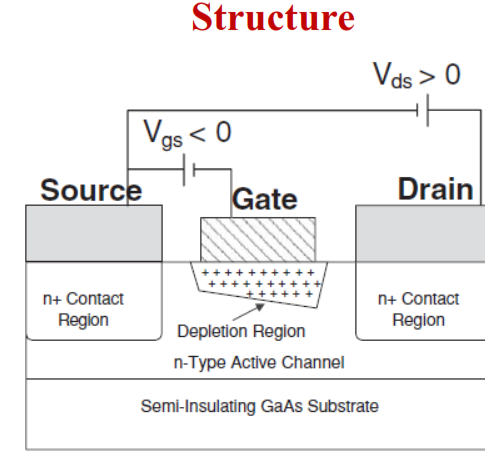
\includegraphics[width=0.48\linewidth]{figs/c4_mesfet.png}\hfill
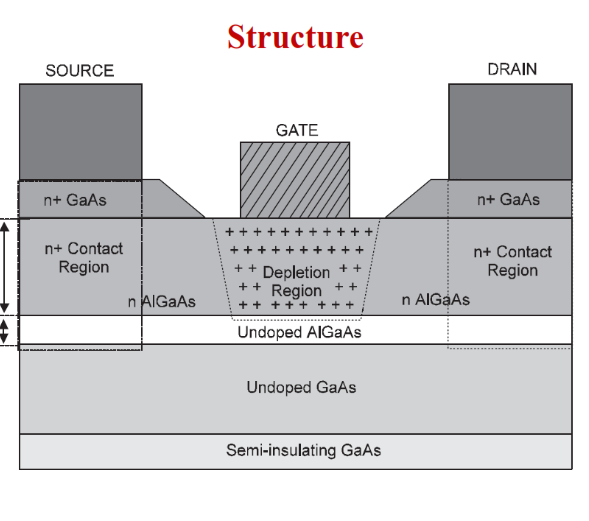
\includegraphics[width=0.48\linewidth]{figs/c4_hemt.png}
{\color{sub}\scriptsize MESFET (left) and HEMT (right) cross-sections. Gangaju slides 85 and 86.}}

\penalty0\vspace{2pt}

%=======================================================================
\T{4.10 Attenuators, Terminations, Windows, Microstrip}

\Q{Microstrips}{\m{5}}
{\color{sub}\footnotesize \tP{1} \yr{\textbf{69 Bh}} \gap$\cdot$\gap geometry and microstrip vs strip-line are in $\S$1.6; stub realisation in $\S$2.9}
\begin{itemize}
  \item Strip of width $W$ on a substrate of thickness $h$ and permittivity $\epsilon_r$,
    ground plane underneath, air above.
  \item \textbf{Quasi-TEM}: the field lives partly in air and partly in the substrate, so it
    sees an effective permittivity
    $\epsilon_{\text{eff}} = \dfrac{\epsilon_r + 1}{2} + \dfrac{\epsilon_r - 1}{2}\dfrac{1}{\sqrt{1 + 12h/W}}$,
    $1 < \epsilon_{\text{eff}} < \epsilon_r$.
  \item $v_p = c/\sqrt{\epsilon_{\text{eff}}}$, $\lambda_g = \lambda_0/\sqrt{\epsilon_{\text{eff}}}$;
    $Z_0$ falls as $W/h$ rises.
  \item (+) planar, cheap photolithography, components mount on top, MMIC friendly.
  \item (-) radiation at bends, dispersion, lower Q and power than waveguide, crosstalk.
\end{itemize}

\par\penalty0\Needspace{14\baselineskip}
\sbsr{0.58}{%
\lead{Attenuators and terminations (syllabus, not yet asked)}
\begin{itemize}
  \item \textbf{Attenuator}: reduces power by a set amount with low VSWR; a resistive
    (carbon) vane or flap in the guide absorbs power through induced currents.
  \begin{itemize}
    \item \textbf{Fixed}: lossy vane, or lossy walls.
    \item \textbf{Variable}: \textbf{flap} lowered through a slot in the centre of the
      broad wall (deeper $=$ more loss, since E is strongest there), \textbf{vane} moved
      from side wall to centre, or \textbf{rotary} vane in a circular guide.
  \end{itemize}
  \item \textbf{Matched termination}: absorbs all incident power; a guide section ending in
    a \textbf{tapered} absorbing wedge so the impedance changes gradually and nothing
    reflects.
  \item Reference \textbf{short}: a metal plate; \textbf{sliding short}: movable, sets a
    reactance.
\end{itemize}}{%
\figT{c4_attenuator.png}
{\color{sub}\scriptsize Flap and rotating-vane attenuators. Gangaju slide 39.}
\lead{Windows, posts and screws (waveguide matching)}
\begin{itemize}
  \item \textbf{Inductive window}: diaphragms from the \textbf{side} walls $\rightarrow$
    shunt L.
  \item \textbf{Capacitive window}: from \textbf{top and bottom} $\rightarrow$ shunt C;
    limits power (breakdown).
  \item \textbf{Resonant window}: both $\rightarrow$ parallel LC, transparent at resonance.
  \item \textbf{Post / screw}: part-way in $\rightarrow$ capacitive; right through
    $\rightarrow$ inductive; $\lambda/4$ deep $\rightarrow$ series resonance.
  \item Waveguide equivalent of a stub ($\S$2.6).
\end{itemize}}

\penalty0\vspace{2pt}

%=======================================================================
\T{4.11 PYQ Mapping}

\lead{Theory questions, covered in this document}
\begin{itemize}
  \item \textbf{Rectangular waveguide field equations, TE mode} $\rightarrow$ $\S$4.1.
    \yr{\textbf{70 Bh} \m{7}, 74 Ma \m{4}, \textbf{77 Ch} \m{8}, \textbf{79 Ch} \m{10},
    \textbf{80 Ch} \m{10}, \textbf{\texttt{80 Bh}} \m{4}}
  \item \textbf{Rectangular waveguide field equations, TM mode} $\rightarrow$ $\S$4.1.
    \mk{Most repeated topic of the chapter, with the TE list: 14 papers.}
    \yr{70 Ma \m{7}, \textbf{71 Bh} \m{8}, 72 Ma \m{5}, \textbf{74 Bh} \m{10},
    \textbf{76 Bh} \m{10}, \texttt{81 Ba} \m{8}, \textbf{\texttt{81 Bh}} \m{8}}
  \item \textbf{Rectangular waveguide: modes of propagation and critical parameters}
    $\rightarrow$ $\S$4.1 Step 6 and $\S$4.2. \yr{\textbf{69 Bh} \m{8}}
  \item \textbf{Prove TM$_{01}$ / TM$_{10}$ do not exist} $\rightarrow$ $\S$4.2. \yr{70 Ma \m{3}}
  \item \textbf{Lowest TM mode is TM$_{11}$} $\rightarrow$ $\S$4.2. \yr{\textbf{\texttt{82 Bh}} \m{3}}
  \item \textbf{TE$_{10}$ dominant; TE$_{10}$ vs TE$_{20}$} $\rightarrow$ $\S$4.2, with the
    81 Bh inequality defect. \yr{\textbf{71 Bh} \m{2}, \textbf{\texttt{81 Bh}} \m{3}}
  \item \textbf{Dominant and degenerate modes; $a = 3b$} $\rightarrow$ $\S$4.2 and
    companion Problem 4. \yr{\textbf{72 Ash} \m{5}, 72 Ma \m{2+2}, \texttt{82 Ba} \m{3}}
  \item \textbf{Circular waveguide, TE / TM field equations, TE vs TM, dominant mode}
    $\rightarrow$ $\S$4.3. \yr{71 Ma \m{10}, \textbf{75 Bh} \m{8+2}, \textbf{\texttt{79 Bh}} \m{10},
    \texttt{82 Ba} \m{7}}
  \item \textbf{Probe vs loop coupling} $\rightarrow$ $\S$4.4. \yr{\textbf{69 Bh} \m{5}}
  \item \textbf{Magic tee: principle, S-parameters, derivation} $\rightarrow$ $\S$4.5 and
    $\S$3.6. \yr{71 Ma \m{5}, \textbf{71 Bh} \m{5}, \textbf{72 Ash} \m{3+3}, 72 Ma \m{6},
    \textbf{79 Ch} \m{5}, \textbf{\texttt{79 Bh}} \m{4}, \textbf{80 Ch} \m{5},
    \textbf{\texttt{80 Bh}} \m{4}}
  \item \textbf{Magic tee with both arms shorted} $\rightarrow$ $\S$3.6.
    \yr{\textbf{\texttt{82 Bh}} \m{4}}
  \item \textbf{E-plane vs H-plane tee} $\rightarrow$ $\S$4.5. \yr{\textbf{69 Bh} \m{5}, \texttt{80 Ba} \m{4}}
  \item \textbf{Hybrid tee; terminated E, H, co-planar arms} $\rightarrow$ $\S$4.5 and
    companion Problem 7. \yr{70 Ma \m{8}, \texttt{82 Ba} \m{4+4+2}}
  \item \textbf{Two magic tees joined at E-arms / in H-plane} $\rightarrow$ $\S$4.5 and
    companion Problems 6 and 8. \yr{\textbf{77 Ch} \m{10}, \textbf{78 Ch} \m{5}}
  \item \textbf{3-port directional coupler, S-parameter analysis} $\rightarrow$ $\S$4.5,
    $\S$3.5. \yr{\textbf{75 Bh} \m{4}}
  \item \textbf{Directional couplers; four performance parameters} $\rightarrow$ $\S$4.6.
    \yr{\textbf{73 Bh} \m{6}, \textbf{79 Ch} \m{5}, \texttt{80 Ba} \m{4}}
  \item \textbf{Circulators} $\rightarrow$ $\S$4.7. \yr{\textbf{70 Bh} \m{5}, \textbf{72 Ash} \m{5}, 73 Ma \m{5}}
  \item \textbf{Cavity resonators} $\rightarrow$ $\S$4.8. \yr{74 Ma \m{4}, \textbf{74 Bh} \m{6}}
  \item \textbf{Gunn diode} $\rightarrow$ $\S$4.9. \yr{\textbf{\texttt{79 Bh}} \m{4}}
  \item \textbf{MASER} $\rightarrow$ $\S$4.9. \yr{\texttt{80 Ba} \m{4}}
  \item \textbf{Microstrips} $\rightarrow$ $\S$4.10 and $\S$1.6. \yr{\textbf{69 Bh} \m{5}}
\end{itemize}

\lead{Numerical content}
\begin{itemize}
  \item \textbf{This chapter has a numerical companion}, \textit{Ch4 - RF Microwave Components
    and Devices - Numerical Problems and Solutions}: rectangular-guide parameters
    (\texttt{80 Ba}, 77 Ch), cut-off checks (70 Bh, \texttt{80 Bh}), mode ranking (72 Ma),
    circular-guide cut-offs (75 Bh), and the junction problems (77 Ch, 78 Ch,
    \texttt{82 Ba}).
\end{itemize}

\lead{Syllabus topics never asked in 24 papers}
\begin{itemize}
  \item Termination, phase shifter, attenuators, microwave transistor. Each has a short
    band above ($\S$4.7, $\S$4.9, $\S$4.10) sized for a 4-mark short note.
\end{itemize}

\lead{Errors in the sources, corrected here}
\begin{itemize}
  \item Deck slide 18: $k_y = n\pi/a$ should be $n\pi/b$.
  \item Deck slide 22: figure caption gives the wrong guide size (it is 5 cm $\times$ 2 cm).
  \item Deck slide 72: Gunn low-field current is not a valence-to-conduction transition.
  \item Deck slide 77: a MASER is a quantum device, not a semiconductor device.
  \item Waveguide.pdf p11: TM $E_\phi$ has a minus sign.
  \item Paper 81 Bh Q3a: TE$_{10}$ is dominant when $a > b$, not $b > a$.
\end{itemize}
